\documentclass{beamer}

\usepackage[orientation=landscape,size=a0,scale=1.4,debug]{beamerposter}
\mode<presentation>{\usetheme{mlr}}

\usepackage[sfdefault]{roboto}
\usepackage{roboto-mono}
\usepackage[T1]{fontenc}
\usepackage[utf8]{inputenc} % UTF-8
\usepackage[english]{babel} % Language
\usepackage{hyperref} % Hyperlinks
\usepackage{ragged2e} % Text position
\usepackage[export]{adjustbox} % Image position
\usepackage[most]{tcolorbox}
\usepackage{listings} % for R code
\lstset{language=R,
    basicstyle=\small\ttfamily,
    stringstyle=\color{DarkGreen},
    otherkeywords={0,1,2,3,4,5,6,7,8,9},
    morekeywords={TRUE,FALSE},
    deletekeywords={data,frame,length,as,character},
    keywordstyle=\color{blue},
    commentstyle=\color{DarkGreen}
}
\hypersetup{
    hyperfootnotes=false,
    colorlinks=true,
	linktocpage=true,
	pdfauthor={mlr-org team},
    %linkcolor=[RGB]{3,99,142}, % mlr blue
    urlcolor=[RGB]{231,138,69}
}

\title{Dataflow programming with mlr3pipelines :\,: CHEAT SHEET} % Package title in header, \, adds thin space between ::

\newlength{\columnheight} % Adjust depending on header height
\setlength{\columnheight}{84cm} 

\newtcolorbox{codebox}{%
	sharp corners,
	leftrule=0pt,
	rightrule=0pt,
	toprule=0pt,
	bottomrule=0pt,
	hbox}

\newtcolorbox{codeboxmultiline}[1][]{%
	sharp corners,
	leftrule=0pt,
	rightrule=0pt,
	toprule=0pt,
	bottomrule=0pt,
	#1}

\newtcolorbox{codeboxinline}{%
	sharp corners,
	leftrule=0pt,
	rightrule=0pt,
	toprule=0pt,
	bottomrule=0pt,
	hbox,
	nobeforeafter,
	tcbox raise base}

\newcommand{\codeinline}[1]{\begin{codeboxinline}#1\end{codeboxinline}}

\begin{document}
\begin{frame}[fragile]{}
	\begin{columns}
		\begin{column}{.245\textwidth}
			\begin{beamercolorbox}[center]{postercolumn}
				\begin{minipage}{.98\textwidth}
					\parbox[t][\columnheight]{\textwidth}{
						\begin{myblock}{Intro}
              The mlr3pipelines package is an extension for the \href{https://github.com/mlr-org/mlr3}{mlr3} package and provides so-called \codeinline{PipeOp}s (pipeline operators) which can then be connected with directed edges in a \codeinline{Graph}.
            \end{myblock}
						\begin{myblock}{PipeOps}
              A \codeinline{PipeOp} builds on R6 classes and represents transformative operations on input leading to output but behaves differently during a ``training phase'' and ``prediction phase''. %While the training phase will typically generate a certain model that is saved as an internal state, the prediction phase will operate on the input data depending on the trained model.
              \ \\
              \ \\
              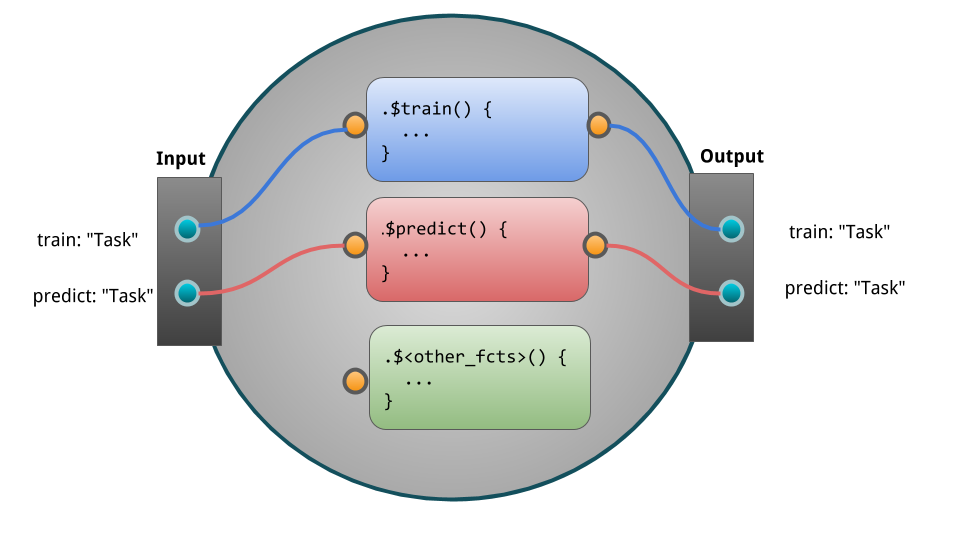
\includegraphics[width=\textwidth]{img/po_viz.png}
              Important \codeinline{PipeOp}s:
              \begin{itemize}
                \item Data Transformer: \codeinline{PipeOpPCA}
                \item Feature Selection: \codeinline{PipeOpFilter}
                \item Repair Tasks: \codeinline{PipeOpRemoveConstants}
                \item Factor Encoding: \codeinline{PipeOpEncode}
                \item Imbalanced Data: \codeinline{PipeOpClassBalancing}
                \item Missing Data: \codeinline{PipeOpImputeHist}
                \item Any Learner: \codeinline{PipeOpLearner}
                \item Ensembles: \codeinline{PipeOpLearnerCV}
              \end{itemize}
              \ \\
              Full list: \codeinline{as.data.table(mlr\_pipeops)} \\
              \ \\
              Construction via a \codeinline{.key}: \codeinline{pca = po("pca")} \\
              \ \\
              Important methods and slots:
              \begin{itemize}
                \item \codeinline{\$train()}
                \item \codeinline{\$predict()}
                \item \codeinline{\$state}
              \end{itemize}
						\end{myblock}
						\vfill}
				\end{minipage}
			\end{beamercolorbox}
		\end{column}
		\begin{column}{.245\textwidth}
			\begin{beamercolorbox}[center]{postercolumn}
				\begin{minipage}{.98\textwidth}
					\parbox[t][\columnheight]{\textwidth}{
						\begin{myblock}{Graphs}
              A \codeinline{Graph} is an instance of an R6 class, collecting \codeinline{PipeOp}s with edges mandating that data should be flowing along them. Edges always pass between \codeinline{PipeOp} \codeinline{channels}.
              \\
              \\
              %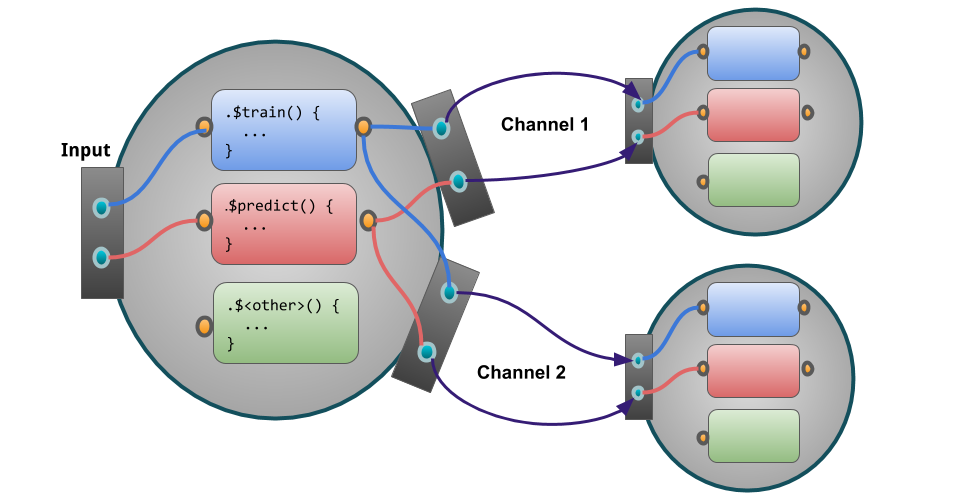
\includegraphics[width=\textwidth]{img/po_multi_viz.png}
              Construction (empty): \codeinline{gr = Graph\$new()} \\
              \ \\
              Adding \codeinline{PipeOp}s:
              \begin{codeboxmultiline}[width=20cm]
                gr\$add\_pipeop(pca)\\
                gr\$add\_pipeop(lrn("classif.rpart"))
              \end{codeboxmultiline}
              \ \\
              Connecting the \codeinline{PipeOp}s:
              \begin{codebox}
                gr\$add\_edge("pca", "classif.rpart")
              \end{codebox}
              \ \\
              Printing and plotting the \codeinline{Graph}:
              \begin{codeboxmultiline}[width=13cm]
                print(gr)\\
                gr\$plot(html = TRUE)
              \end{codeboxmultiline}
              \ \\
              Assessing the \codeinline{PipeOp}s: \codeinline{gr\$pipeops} \\
              \ \\
              A \codeinline{Graph} itself has a \codeinline{\$train()} and \codeinline{\$predict()} method that accept data and propagate this data through the network of \codeinline{PipeOp}s. The return value corresponds to the output of the \codeinline{PipeOp} outputs that are not connected to other \codeinline{PipeOp}s.\\
              \ \\
              Building a linear \codeinline{Graph} like above is much easier using the \codeinline{\%>>\%} operator.
						\end{myblock}
            \begin{myblock}{Syntactic Sugar}
              \codeinline{\%>>\%} takes either a \codeinline{PipeOp} or a \codeinline{Graph} on each of its sides and connects all outputs of its left-hand side to the inputs of its right-hand side:
              \begin{codebox}
                gr = pca \%>>\% lrn("classif.rpart")
              \end{codebox}
              \ \\
              \codeinline{gunion()} arranges them next to each other in a disjoint graph union:
              \begin{codeboxmultiline}[width=19cm]
                gunion(list(po(.key1), po(.key2)))
              \end{codeboxmultiline}
						\end{myblock}
						\vfill}
				\end{minipage}
			\end{beamercolorbox}
		\end{column}
		\begin{column}{.245\textwidth}
			\begin{beamercolorbox}[center]{postercolumn}
				\begin{minipage}{.98\textwidth}
					\parbox[t][\columnheight]{\textwidth}{
            \begin{myblock}{Syntactic Sugar}
              To build a \codeinline{Graph} from layers, use the \codeinline{\%>>\%} operator. It takes either a \codeinline{PipeOp} or a \codeinline{Graph} on each of its sides and connects all of the outputs of its left-hand side to the inputs of its right-hand side:
              \begin{codeboxmultiline}[width=18cm]
                mlr\_pipeops\$get(.key1) \%>>\%
                \hspace*{1ex}mlr\_pipeops\$get(.key2)
              \end{codeboxmultiline}
              \ \\
              The \codeinline{gunion()} operator takes \codeinline{PipeOp}s and \codeinline{Graph}s and arranges them next to each other creating a disjoint graph union:
              \begin{codeboxmultiline}[width=22cm]
                gunion(list(mlr\_pipeops\$get(.key1),\\
                \hspace*{1ex}mlr\_pipeops\$get(.key2))
              \end{codeboxmultiline}
						\end{myblock}
						\begin{myblock}{Learners in Graphs}
              A \codeinline{PipeOpLearner} takes any mlr3 \codeinline{Learner} and produces a \codeinline{PipeOp}. This \codeinline{PipeOp} can be used after a preprocessing pipeline:
              \begin{codeboxmultiline}[width=16cm]
                mlr\_pipeops\$get("learner",\\
                \hspace*{1ex}"mlr\_learners\$get(.key))
              \end{codeboxmultiline}
            \end{myblock}
						\begin{myblock}{Graphs in Learners}
              Dual to this procedure, a \codeinline{Graph} can be wrapped in a \codeinline{Learner}, resulting in a \codeinline{GraphLearner}:
              \begin{codebox}
                grl = GraphLearner\$new(gr)
              \end{codebox}
            \end{myblock}
            \begin{myblock}{Graphs and Predictions}
              When predicting from a \codeinline{Graph} you have to set the predict type of the \codeinline{GraphLearner} explicitly, i.e.:
              \begin{codebox}
                grl\$predict\_type = "prob"
              \end{codebox}
            \end{myblock}
						\vfill}
				\end{minipage}
			\end{beamercolorbox}
		\end{column}
    \begin{column}{.245\textwidth}
			\begin{beamercolorbox}[center]{postercolumn}
				\begin{minipage}{.98\textwidth}
					\parbox[t][\columnheight]{\textwidth}{
            \begin{myblock}{Hyperparameters}
              mlr3pipelines relies on the paradox package to provide parameters that can modify a \codeinline{PipeOp}'s behavior. To inspect the parameters use:
              \begin{codebox}
                mlr\_pipeops\$get(.key)\$param\_set
              \end{codebox}
              \ \\
              To set or retrieve a parameter, the \codeinline{\$param\_set\$values} slot can be accessed. Alternatively, \codeinline{param\_vals} can be specified during construction:
              \begin{codeboxmultiline}[width=17cm]
                mlr\_pipeops\$get(.key,\\
                \hspace*{1ex}param\_vals = list(.values)
              \end{codeboxmultiline}
              \ \\
              Note that in a \codeinline{Graph}, the parameters of all \codeinline{PipeOp}'s are collected together.
              Finally, note that both a \codeinline{PipeOpLearner} and \codeinline{GraphLearner} preserve parameters of the objects they encapsulate.
            \end{myblock}
						\vfill}
				\end{minipage}
			\end{beamercolorbox}
		\end{column}
	\end{columns}
\end{frame}
\end{document}
